\documentclass[10pt]{article}
\usepackage[margin=0.5in]{geometry}
\usepackage{hyperref}
\usepackage{xcolor}
\usepackage{lmodern}
\usepackage{microtype}
\usepackage{tikz}
\usetikzlibrary{arrows.meta,positioning,shapes.geometric,fit}

\hypersetup{colorlinks=true, linkcolor=blue, urlcolor=blue, citecolor=blue}

\makeatletter
\renewcommand{\section}{\@startsection{section}{1}{0pt}{0.4ex plus 0.1ex}{0.15ex}{\normalfont\bfseries}}
\makeatother

\setlength{\parskip}{0.15em}
\setlength{\parindent}{0em}
\pagestyle{empty}
\sloppy

\begin{document}
\small

\begin{center}
{\bfseries DSO Concept Outline --- Metastable L1$_2$/D0$_{22}$ Strengthening Phases in Rapidly Solidified Dilute Al-MPEAs Inaccessible to Equilibrium CALPHAD}
\end{center}

{\small \textbf{PI:} Sterling Baird (Brigham Young University, Materials Science \& Engineering). \textbf{Solicitation:} DARPA DSO Office-Wide BAA (1-page exec summary $\to$ invited full proposal); adjacent to METALS, SURGE. \textbf{Type:} seedling \$0.5--1M / 12--18~mo, with Phase~1 follow-on \$2--4M / 24~mo. \textbf{Keywords:} non-equilibrium phase selection, metastable L1$_2$, dilute Al-MPEA, BOFN, LPBF.}

% Shared FLAIME pipeline DAG used by all three concept outlines.
% Requires \usepackage{tikz} and \usetikzlibrary{arrows.meta,positioning,shapes.geometric,fit}
\begin{center}
\resizebox{\textwidth}{!}{%
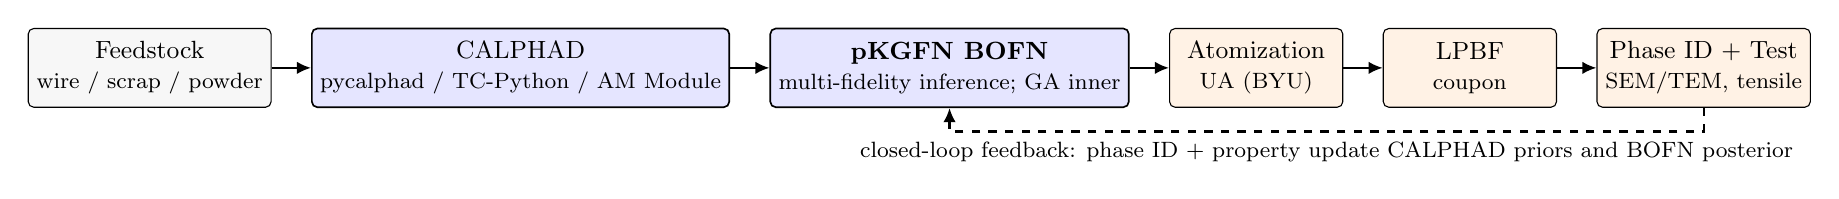
\begin{tikzpicture}[
    node distance=4.5mm and 5mm,
    every node/.style={font=\small},
    block/.style={rectangle, draw, rounded corners=2pt, align=center,
                  minimum height=10mm, minimum width=22mm, inner sep=3pt,
                  fill=black!3},
    ai/.style={block, fill=blue!10, line width=0.6pt},
    expt/.style={block, fill=orange!10},
    arr/.style={-{Latex[length=1.8mm,width=1.6mm]}, thick}
]
  \node[ai] (cal) {CALPHAD\\\footnotesize{pycalphad / TC-Python / AM~Module}};
  \node[ai, right=of cal] (bofn) {\bfseries pKGFN BOFN\\\footnotesize{multi-fidelity inference; GA inner}};
  \node[block, left=of cal] (feed) {Feedstock\\\footnotesize{wire / scrap / powder}};
  \node[expt, right=of bofn] (ua) {Atomization\\\footnotesize{UA (BYU)}};
  \node[expt, right=of ua] (lpbf) {LPBF\\\footnotesize{coupon}};
  \node[expt, right=of lpbf] (test) {Phase ID + Test\\\footnotesize{SEM/TEM, tensile}};
  \draw[arr] (feed) -- (cal);
  \draw[arr] (cal) -- (bofn);
  \draw[arr] (bofn) -- (ua);
  \draw[arr] (ua) -- (lpbf);
  \draw[arr] (lpbf) -- (test);
  % Loop-closure feedback arrow under the row.
  \draw[arr, dashed] (test.south) -- ++(0,-3mm) -| node[below, pos=0.25, font=\footnotesize]
      {closed-loop feedback: phase ID + property update CALPHAD priors and BOFN posterior} (bofn.south);
\end{tikzpicture}%
}
\end{center}


\section*{Fundamental technical barrier}
The DARPA-hard claim is metallurgical, not logistical: \emph{rapid-solidification thermal histories accessible via UA + LPBF stabilize coherent metastable L1$_2$-Al$_3$(Zr,Ti,X) and D0$_{22}$-related ordered nanoprecipitates in dilute Al-Mn-Cr-Zr-Si-Ti space that current CALPHAD assessments rank as thermodynamically inaccessible at the bulk equilibrium level}, and these phases can deliver Al-Ce/Al-Ni-Sc-class elevated-temperature strength without REE/Sc additions. Equilibrium databases predict that Mn/Cr/Zr/Si/Fe additions cannot replicate the L1$_2$/D0$_{22}$ strengtheners that Sc/REE enable; the wager is that quenched-in supersaturation plus rapid LPBF re-melt cycles open a metastable solubility window in which these ordered phases nucleate at $10^4$--$10^6$ K/s cooling rates, and that a closed BOFN-CALPHAD-experiment loop is the only tractable way to navigate that phase space without a combinatorial library. If the claim fails (no L1$_2$/D0$_{22}$-class precipitate observed by TEM/APT, or property delta $< $50\% of comparator), no engineering wrap can rescue the program. Wire/scrap feedstock is downstream transition value, not the proposed DSO risk.

\section*{Idea}
The FLAIME discovery loop --- pKGFN BOFN over CALPHAD multi-fidelity nodes (\texttt{pycalphad}, TC-Python/TCAL10, AM~Module), validated by UA and LPBF --- applied to a constrained dilute Al-MPEA design space (Al + Mn/Cr/Zr/Ti/Si/Fe, $\le$5 active solute elements). The objective function is dominated by (i)~elevated-temperature UTS retention and (ii)~TEM/APT-confirmed presence of the predicted ordered-precipitate family; printability window and feedstock convertibility are constraints, not design targets. \textbf{Hypothesis:} the loop, narrowed to a metastable-L1$_2$/D0$_{22}$ objective, can deliver one alloy candidate end-to-end (BOFN-CALPHAD design $\to$ UA powder $\to$ LPBF coupon $\to$ TEM/APT phase ID + elevated-temperature tensile) within a 12-month seedling, with the alloy occupying a phase region not predicted by current Al-MPEA databases.

\section*{Why DSO (fundamental risk, not integration risk)}
\emph{Risk DSO is positioned to take:} the metallurgical claim that rapid-solidification AM unlocks coherent metastable L1$_2$/D0$_{22}$ ordered nanoprecipitates in dilute Al-MPEA space unreachable by equilibrium thermodynamics. Component pieces (UA atomizer, LPBF baseline, BOFN) exist; their integration is engineering and is not the proposed DSO risk. \textbf{Seedling go/no-go (12~mo):} (i)~one alloy candidate carried BOFN-CALPHAD design $\to$ UA powder $\to$ LPBF coupon $\to$ tensile + TEM/APT; (ii)~independent test article printed at JHU~APL using the resulting powder, characterized at BYU; (iii)~TEM or atom-probe evidence of an L1$_2$- or D0$_{22}$-class precipitate predicted by the loop but absent from baseline CALPHAD assessment of the same composition; (iv)~as-built UTS retention at 200~$^\circ$C $\ge$~85\% of published Al-10Ce-3Ni and Al-2Sc-1Zr datasets at matched product form (LPBF coupon, no T6); (v)~side-by-side public CALPHAD prediction showing the observed strengthening constituent should not exist at the measured cooling-rate history.

\section*{Preliminary results (FLAIME pipeline, BYU, Apr~2026)}
AMAZEMET rePOWDER UA atomizer installed and operating at BYU; SEM/EDS on UA-modified powder (AlSi10Mg + Al wire + Si feed) showing measurable composition shift --- the powder-modification pathway exists in working form. Elevated-temperature tensile data on a standard Al specimen; AlSi10Mg LPBF tensile baseline (printed at U.~Utah Spear lab via no-cost MOU). Working pKGFN BOFN; Thermo-Calc AM~Module simulations on candidate compositions; automated powder dispensing demonstrated.

\section*{Security posture and partnership}
\textbf{Funded:} BYU (Baird, lead --- BOFN, CALPHAD, UA, phase ID, tensile). \textbf{Funded transition partner:} JHU~APL --- independent print of the candidate alloy on an APL LPBF system, plus a transition pathway through APL's existing relationships with AFRL Manufacturing \& Industrial Technologies Division and the Army DEVCOM Armaments Center; APL serves as the FFRDC-style bridge from seedling demonstration to a named DoD program office, not as the end customer. \textbf{Unfunded U.S. collaborator:} U.~Utah Spear lab (no-cost LPBF baseline coupon access via existing MOU). Work is performed at BYU and APL on unclassified, fundamental-research-basis data (NSDD-189); no CUI/ITAR data are anticipated in the seedling. If a Phase~1 follow-on requires CUI handling, BYU has an established research-security office; APL operates at the required posture and would host any controlled data. \textbf{Adjacent venues acknowledged:} pure logistics-integration framings of this work are better placed at ONR (Naval Materials Division), Army DEVCOM, or DLA; the DSO submission is reserved for the fundamental metallurgical claim above.

\section*{Scope separation from pending DOE Genesis Mission Topic~3B and request}
\textbf{Task-level scope separation.} \emph{Genesis tasks (DOE-funded):} alloy-agnostic platform construction --- hardware/software integration, scheduler, data fabric, autonomous orchestration, general platform validation across broad composition/process spaces. \emph{DSO seedling tasks (this proposal):} (T1)~hypothesis-bound CALPHAD-BOFN study scoped to the L1$_2$/D0$_{22}$ ordered-precipitate question in a defined dilute Al-MPEA window; (T2)~powder + coupon production for the named candidate; (T3)~TEM/APT phase ID and elevated-temperature tensile against published Al-Ce/Al-Ni-Sc benchmarks; (T4)~independent APL print + characterization. Personnel labor, deliverables, data packages, and reporting artifacts are itemized separately; no scheduler or platform-development task appears in both. \textbf{Request:} a read on a 1-page exec summary before we invest in a full proposal.

{\small \emph{Repository and full vision:} \url{https://github.com/vertical-cloud-lab}.}

\end{document}
